\RequirePackage[l2tabu, orthodox]{nag}

\documentclass{article}

	\usepackage[a4paper]{geometry}
	\usepackage{fullpage}
	\usepackage{graphicx}
	\usepackage{siunitx}
		\sisetup{separate-uncertainty}
	\usepackage{url}
	\usepackage[title]{appendix}
	\usepackage{microtype}
	\usepackage[colorlinks=false, pdfborder={0 0 0}]{hyperref}
	
	\usepackage[backend=bibtex,sorting=none]{biblatex}
		\bibliography{../bib/biblo,../bib/cust} %Insert Bibliography file name
	\setlength\parindent{0pt}
	\usepackage{subcaption}
	\usepackage{float} 
	\usepackage{commath}
	\usepackage{amsfonts}
	\usepackage{booktabs}
		\setlength\heavyrulewidth{1.5pt}
	\usepackage[capitalise]{cleveref}
	\usepackage{pgfgantt}
	\usepackage{rotating}
	

	

%Document information

\title{Fast Simulation of Particle Physics Detectors Using Machine Learning Tools: Initial Report}

\author{Seyon \textsc{Sivarajah}, Churchill College, ss2165}

\date{\today}

%End Document information

\begin{document}
\maketitle


\begin{center}
\begin{tabular}{lr}

%Experiment Performed: &  \\

Supervisor: & Dr Christopher Lester\\

%Experiment Title: & 
\end{tabular}
\end{center}


%------------------ABSTRACT-------------------

\begin{abstract}
A key part of experimental particle physics is the simulation of a detector's response to an event. This initial report outlines the background and plans for an investigation into the possibility of using machine learning tools, and neural networks in particular, to learn and generate such simulated data. State of the art accurate simulators are slow and computationally expensive, a successful generative network could lead to a significant performance increase at manageable accuracy costs. This investigation is an attempt at a demonstration of this concept.
\end{abstract}

%------------------Introduction-------------------
\section{Introduction}

Particle physics experiments involve colliding particles and measuring the properties of the objects produced. However, a given event could not only result in a variety of particle showers, but the response of the detector is also stochastic in nature. It is from this determination of track properties and object momenta that a physicist must infer the original event. Detector simulations are widely used to help with the inference by calculating what a response and output for a given event would be, and as such can be used as predictive tools for models.\\

Full, accurate simulations (AS) of the progress of particles through detectors, such as the commonly used Geant 4 \cite{geant4}, can produce extremely accurate predictions of the measurements. However, they are computationally expensive. Approximate, fast simulators (FS), such as Delphes \cite{delphes}, perform cruder calculations with a significant speed gain (AS $\sim$ 10-1000s/event and FS $\sim$ 0.01-1s/event \cite{delphessl}). The accuracy-performance imbalance between these two solutions leaves room for other potential avenues. One such route is the use of machine learning tools which have shown notable promise in a large number of fields.\\

Generative models attempt to learn a given probability distribution via exposure to samples, and thus accurately generate new elements of that distribution. Their capability has recently been significantly boosted by the burgeoning fields of neural networks and associated deep learning. Once the learning process is complete, such networks are demonstrably fast for appropriate usage. As such, a generative model capable of learning to simulate detector responses may strike a better performance-accuracy balance than current FS. \\

This research project initially focusses on attempting a proof of this concept using Generative Adversarial Networks (GANs) \cite{gan1}. This method trains two networks simultaneously, a generative model $G$ and discriminative model $D$. As the names suggest, G generates ``fake" data which D attempts to distinguish from the ``real" training data. As each network is trained to improve at their task, they compete such that ultimately G produces new data which is indistinguishable in theory from the original distribution.\\

This investigation would train using simulated data from a FS, aiming to match the accuracy of said simulator while surpassing in performance. A successful demonstration merits further work to attempt closer accuracy to AS. The following section gives the relevant background on particle detectors, simulations and machine learning tools. \cref{sec:plan} outlines the project plan, including methods, challenges and tasks.

%------------------Theory-------------------
\section{Background}
\label{sec:background}



\subsection{Detectors \& Simulations}
\label{sec:detector}

\begin{figure}[H]
	\centering
	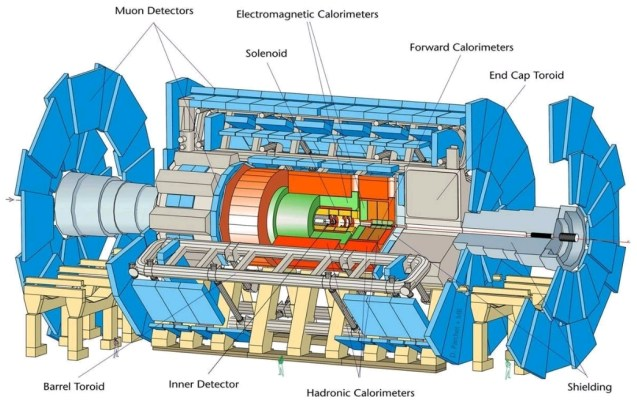
\includegraphics[width=0.8\linewidth]{img/atlasdetector}
	
	\caption{Cutaway diagram showing components of ATLAS detector. Source: \cite{atlaspic}}
	\label{fig:atlaspic}
	
\end{figure}


Modern particle detectors are a complex set of measurement systems working in unison. Taking as an example the ATLAS experiment, we can see in \cref{fig:atlaspic} a cutaway of the detector set up. Simplistically, the energy and momentum of particles travelling out from the collision are measured by the calorimeters. The solenoids create a controlled magnetic field, the direction of travel in the field and the curvature of the particles gives a measurement of charge and mass respectively. A detailed description of the detector can be found in \cite{armstrong}.
\\


The response of a detector to a particular particle event is therefore non-trivial to predict, particularly due to the high degree of stochastic variation between any two measurements. A significant difficulty faced by LHC experiments is the jets of hadronisation produced by quarks or gluons, as only the final branches of the jets are measured by the calorimeters. Without an understanding of this response, however, a physicist cannot infer the event that took place, or indeed make predictions about measurements that will be made. It is in this arena that simulations of detector behaviour are crucial. \\

\cref{fig:simdiag} outlines a typical simulation sequence. The first step in the process is a matrix element calculator, which for this investigation is the commonly used MadGraph5 \cite{madgraph}. This piece of software loads a given model (particles and interactions), and calculates all the tree-level diagrams which take the given initial particles to the final particles. Using this information, Monte-Carlo methods are used to calculate the matrix element using a given number of events. Next, an event generator, Pythia for our case, calculates the subsequent interactions, decays parton showers and hadronisation \cite{Gieseke2012}.\\

The results of this are the``truth events", which for our purposes is the input, $\mathbf{x}$, to any simulator under consideration. The simulator performs two key tasks, that of calculating the response of the detector as the particles travel through it, and reconstructing the underlying events from such information. The reconstruction step is performed in much the same way as actual experiments, so is a useful representation of the simulated results.        

\begin{figure}[H]
	\centering
	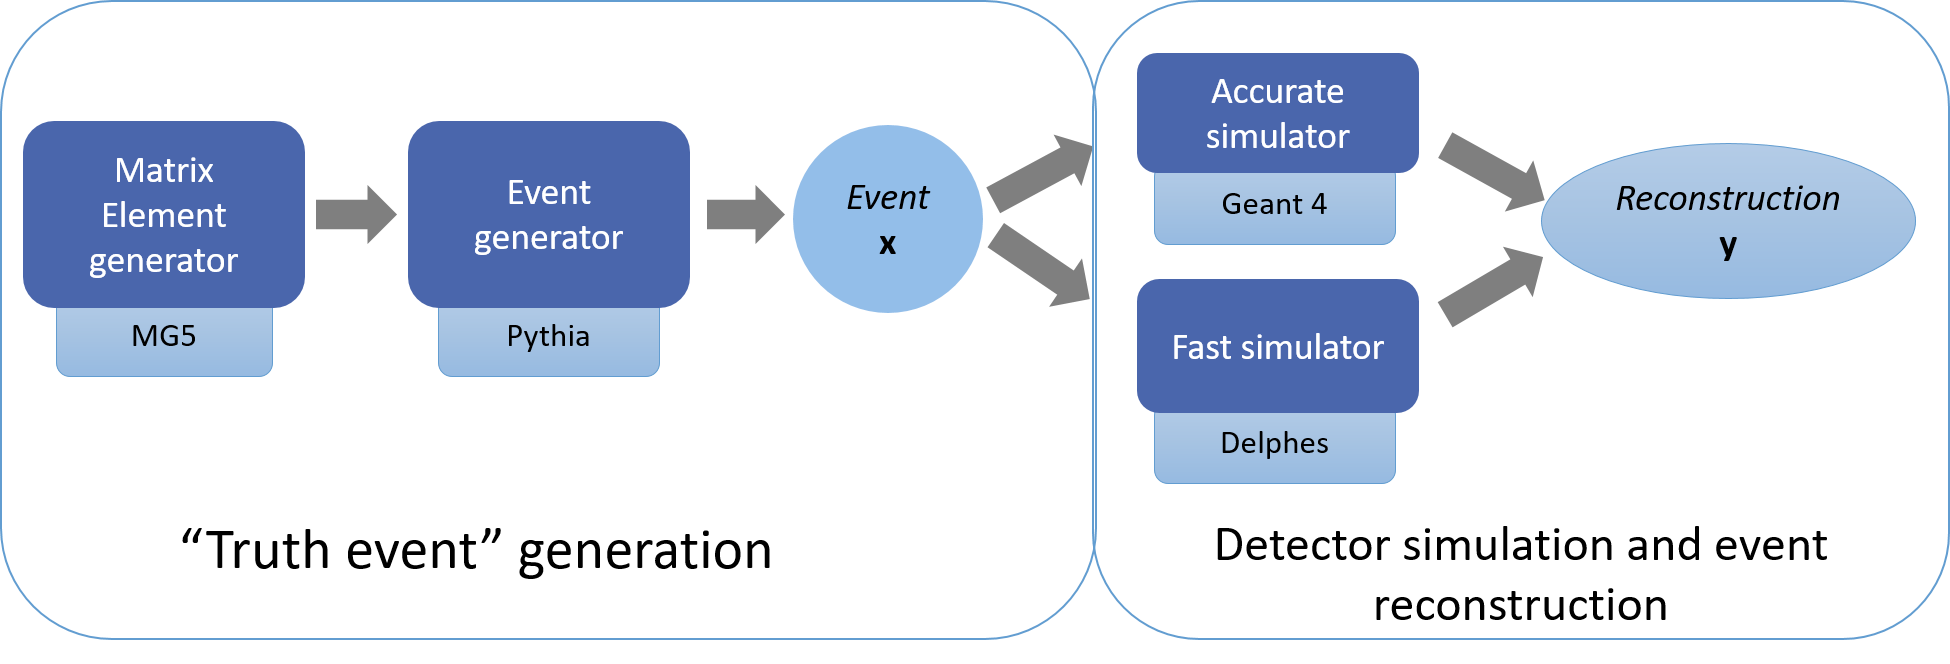
\includegraphics[width=0.8\linewidth]{img/simdiag}
	
	\caption{Summary of simulation process, from matrix element generation to final reconstruction from detector response.}
	\label{fig:simdiag}
	
\end{figure}	


An AS then propagates the input through a detailed model of the detectors to calculate the response. Delphes, the FS under consideration, takes a modular approach by separating the various components of the detector and performing approximate calculation and addition of stochasticity at each stage. Details of this can be found in \cite{delphes}. A measure of the performance of various parts can be seen in \cref{fig:delphescpu}. The FastJet jet propagation \cite{fastjet} is by far the slowest, especially at high pile-up (multiple simultaneous proton-proton interactions \cite{marshall}). Any performance improvements are likely to arise from better execution of this step. \\ 


\begin{figure}[H]
	\centering
	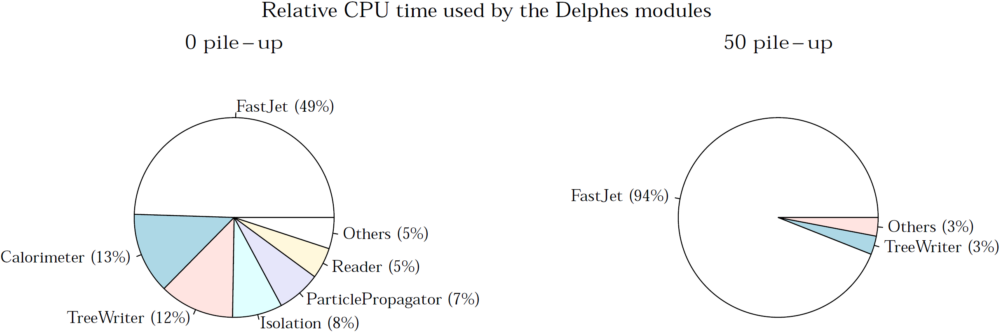
\includegraphics[width=0.7\linewidth]{img/delphescpu}
	
	\caption{Performance of Delphes modules at 0 and 50 pile-up. FastJet jet propagation algorithm is seen to be most costly, especially at high pile-up. Source: \cite{delphes}}
	\label{fig:delphescpu}
	
\end{figure}

 
\subsection{Machine Learning}
\label{sec:ml}

Traditional and well developed machine learning can be understood very much in parallel with the Bayesian methods of experimental physics. We attempt to determine the most likely parameters, $\theta$, for a given model, $\mathcal{M}$, for measurements $y$. This probability, $p(\theta|y, \mathcal{M})$, is the posterior. It is usually done by maximising the likelihood (probability of data given parameters) \cite{data}:

\[
p(y|\theta, \mathcal{M}) = \frac{p(\theta|y, \mathcal{M})p(y|\mathcal{M})}{p(\theta|\mathcal{M})}
\]

In machine learning, computers perform this task using training data to learn the parameters, then subsequently make predictions on new data. Typically these actions are classification (labelling), regression (common in physics) and clustering (similarity of data points). \\

More recent developments have made significant inroads into \textit{generative} models, wherein learning is done in order to produce new samples of data. In particular neural networks and deep learning have played a large role, as neural networks scale well with dimensions, are end-to-end differentiable (crucial for gradient based training) and can represent complex functions \cite{deepgen}.\\

Generative Adversarial Nets (GANs), proposed by Goodfellow et al. \cite{gan1} have proven very successful in areas such as image generation and text to image synthesis \cites{radford}{text2im}. More recently, it has been shown that GANs can be used to generate particle shower shape data \cite{louppe}, which is promising for our goals. \\

Basic GANs consist of two competing networks $G$ and $D$. $G$ takes a latent noise variable $z$ as input and outputs artificial data $\mathbf{y} = G(z;\theta_g)$, where $\theta_g$ are the parameters of the network. $D$ takes either real or artificial data as input and outputs a scalar, $D(\mathbf{y})$, corresponding to the probability that $\mathbf{y}$ is real. $G$ is trained to improve at fooling $D$ and $D$ is trained to improve at distinguishing real data from generated. This can be described by a min-max game with value function $V(G,D)$:

\begin{equation}
	\label{eq:minmax}
	\min_{G}\max_{D}V(D,G) = \mathbb{E}_{\mathbf{y}\sim p_{\text{data}}(\mathbf{y})} [\log(D(\mathbf{y})] + \mathbb{E}_{\mathbf{z}\sim p_{z}} [\log(1-D(G(z)))] 
\end{equation} 

where  $\mathbb{E}_{\mathbf{y}\sim p_{\text{data}}(\mathbf{y})}$ expresses expectation over the data probability distribution.  \\

It can be shown that there exists a unique solution to this, a saddle point, strictly when $p_{\text{data}} = p_G$, where $p_G$ is the distribution produced by $G$. This theoretical guarantee is a key advantage of GANs, as well as the ability to train them using standard back propagation algorithms and the lack of Markov Chains which are often needed in other generative models.   


%------------------Method-------------------

\section{Project Plan}
\label{sec:plan}


\subsection{Method}
This project aims to apply machine learning methods to simulate particle detectors, beginning with GANs. The first key step is to understand and transform the event into a suitable input for the neural network. Similarly, the reconstructed output of Delphes must be reduced to the crucial parts that $G$ will need to replicate. This is important as the size of the output scales with event number, so could be typically 100s of megabytes, which is large compared to the image file sizes that GANs have mainly been tested on.\\

A key difference between basic GANs and this case is the requirement that the output $\mathbf{y}$ of $G$ match a given input $\mathbf{x}$. $G$ and $D$ must therefore be conditional on the event input. Such conditional use of GANs has been demonstrated \cite{mirza2014conditional}, and it can be shown that a simple modification of \cref{eq:minmax} is sufficient:

\[
 \min_{G}\max_{D}V(D,G) = \mathbb{E}_{\mathbf{y}\sim p_{\text{data}}(\mathbf{y})} [\log(D(\mathbf{y|x})] + \mathbb{E}_{\mathbf{z}\sim p_{z}} [\log(1-D(G(z|\mathbf{x})))] 
\]

Furthermore, appending $\mathbf{x}$ to the input for each net is enough to achieve this. \cref{fig:mldiag} shows this set up.

\begin{figure}[H]
	\centering
	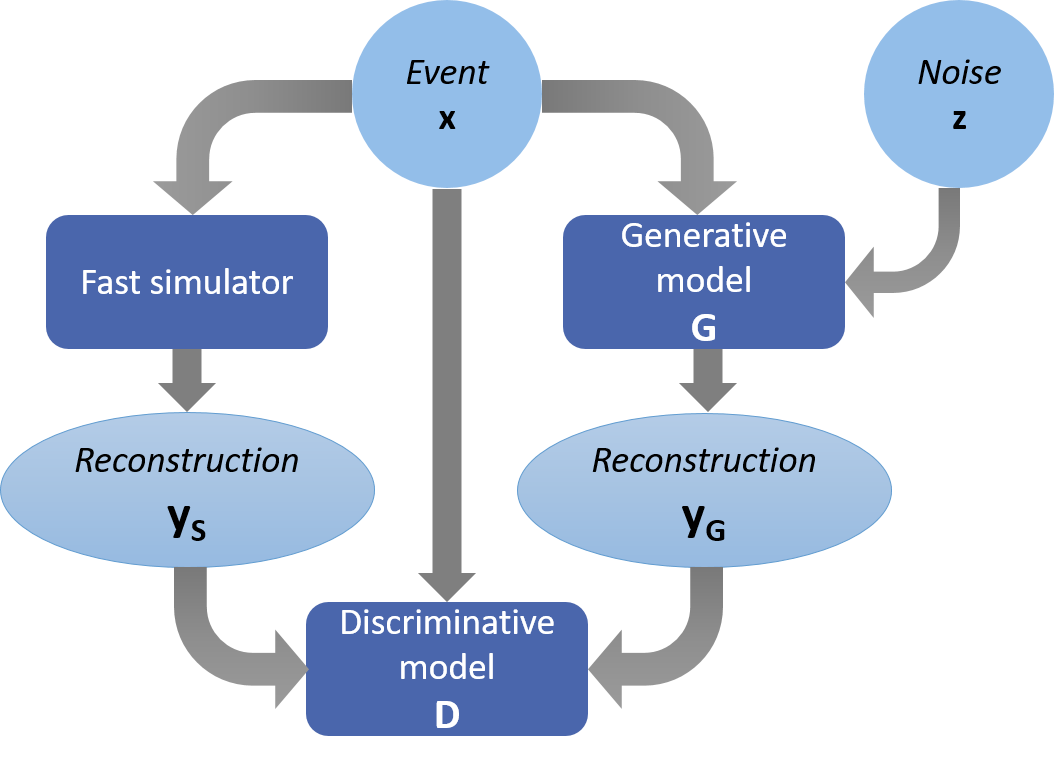
\includegraphics[width=0.6\linewidth]{img/mldiag}
	
	\caption{Schematic of simulation and neural net based generation of data.}
	\label{fig:mldiag}
	
\end{figure}


Initially training will take place with one or a few simple events (e.g. just one or two particles) as input. Eventually the simulation must be made capable of being conditional on any event input.\\

The project will be implemented in Python 2.7, with the associated scientific packages numpy, scipy and matplotlib. The package theano \cite{theano} will be used for optimized calculation and symbolic manipulation, primarily due to its compatibility and support for GPUs, which significantly boost neural net performance. Keras \cite{keras} is a package that simplifies machine learning actions and works on top of theano; it will be the main tool used for constructing the networks and training. The training algorithm will likely be a form of stochastic gradient descent such as ADAM \cite{adam}\\

\subsection{Challenges}

Some expected key challenges are:
\begin{itemize}
	\item The potentially large size of the input, and the large number of inputs which need to be trained for is also an issue. Fortunately, as the training data is simulated, the availability is only limited by computation time. 
	\item The nets based approach will need to be adapted to work with an input size that could vary by orders of magnitude, they typically accept only a fixed length input. 
	\item In the GANs, if $G$ is trained too much without updating $D$, the "Helvetica scenario" arises, where $G$ will map too many $z$ to the same $\mathbf{y}$ \cite{gan1}. This, and the rate of learning, require fine tuning. 
\end{itemize}


\subsection{Tasks}
%\ganttset{bar height=.6}

\begin{figure}[H]
	\begin{center}
		
	\begin{ganttchart}[
		hgrid,
		vgrid,
		x unit=0.5cm,
		y unit title=1cm,
		y unit chart=0.5cm
		]{1}{24}
		\gantttitle{December}{5} \gantttitle{January}{4}\gantttitle{February}{4}\gantttitle{March}{5}\gantttitle{April}{4}\gantttitle{May}{2}\\
		\gantttitlelist{1,...,24}{1}\\
		\ganttgroup{Preliminary}{1}{3} \\
			\ganttbar{Initial Report}{1}{1} \\
			\ganttbar{GAN practice}{1}{3} \ganttnewline
			\ganttbar{Reduce Delphes output}{2}{3}\\

		\ganttgroup{Core Development}{7}{18} \\
			\ganttbar{1 Particle}{7}{8}\\
			\ganttbar{1 Complex event}{9}{11}\\
			\ganttbar{Multiple events}{11}{13}\\
			\ganttbar{Large event No}{13}{16}\\
			\ganttbar{Testing, validation}{16}{18}\\
						
		\ganttgroup{Write-up}{15}{24} \\
			\ganttbar{Presentation}{15}{16}\\
			\ganttbar{First Draft}{15}{21}\\
			\ganttbar{Feedback}{20}{23}\\
			\ganttbar{Final}{22}{24}\\
%		\ganttlink{elem2}{elem3}
%		\ganttlink{elem3}{elem4}
	\end{ganttchart}

	\end{center}
	\caption{Gantt chart of expected work on this project, divided by week.}
\end{figure}

%presentation in lent week 7
% report on 15th May 2017
\newpage
%------------------References-------------------
\printbibliography

\begin{appendices}

\end{appendices}


\end{document}
